\chapter{Solving an exact cover problem using the QAOA} \label{ch:qaoa}
An optimization problem where the aim is to find the optimal (or close to optimal) solution amongst a finite set of possibilities is called a \textit{combinatorial optimization problem}.  Such problems are pervasive and appear in applications such as green logistics, hardware verification, task scheduling and telecommunication network design \cite{Sbihi2007CombinatorialA, Coles2018QuantumBeginners, 2014ApplicationsOptimization}.

In this chapter, we first introduce the notion of combinatorial optimization. Next, we explain the \gls{qaoa}, a quantum heuristic algorithm providing approximate solutions to combinatorial optimization problems. We show that using \glspl{carb} can reduce the length of \gls{qaoa}'s gate sequence implemented on the quantum computer. This allows for more complex algorithms to be run on the quantum computer compared to when only \gls{cz} are used. Next, we demonstrate this advantage experimentally by solving a combinatorial optimization problem called exact cover on a three qubit quantum processor.

\section{Combinatorial optimization}
It its general form, a combinatorial optimization problem is specified by a set of rules, called clauses, acting on strings of $N$ bits, in which each bit represents a binary decision variable \cite{Farhi2014AAlgorithm}.  Each clause is satisfied for certain assignments of the bits and unsatisfied for other assignements. Solving the problem consists in finding a combination of bits (forming together the bit string) satisfying the largest (weighted) amount of clauses. The objective function can be written as 
\begin{equation}
    C(b) = \sum_{m=1}^M w_m C_m(b)
\end{equation}
where $b = b_1 \, ...\, b_N$ the bit string,  $C_m(b)$ is the $m$-th clause and $w_m$ is its corresponding (real and non negative) weight. If $C_m(b)$ is satisfied by the bit string $z$ then its value is 1 and otherwise 0. In these terms, solving the problem is expressed as finding the bit string $b_\text{opt}$ maximizing C. An approximate solution provides a bit string $b_{\text{approx}}$ for which  $C(b_{\text{approx}})$ is close to the maximum of C.

We illustrate this abstract concept with a simple example. Imagine you are going to a party, and have to choose an outfit -- consisting of one t-shirt and one pair of pants -- from your closet. You have 2 shirts to choose from, a black (0) and white (1) one. Similarily, you have a black (0) and a white (1) pair of pants. You believes you look better when your whole outfit is of the same color. Additionally, you  believe your white shirt suits you better than the black one. Which outfit should you choose for the party? 

While the answer is trivial in this example, we formalize the problem with the terminology introduced above. The outfit, $b$, can be formulated as a 2-bit string, one bit for the shirt ($b_1$), and one for the pair of pants ($b_2$). Colors are encoded by the values of the bits: 0 for black and 1 for white. The four possible outfits are: 00 (black-black), 01 (black-white), 10 (white-black) and 11 (white-white). The problem has two clauses. $C_1(b) := b_1 \oplus b_2$, leading to a value of 1 if you choose a shirt and pair of pants of the same color and 0 otherwise\footnote{$\oplus$ denotes the "XOR" operation, which gives an output of 1 if and only if the two inputs are 11 or 00}. $C_2(b) := b_1$ has a value of 1 if you chooses your white shirt. The objective function is then:
\begin{equation}
    C(b) = C_1(b) + C_2(b) = (b_1 \oplus b_2) + b_1
\end{equation}
where we assigned equal weights $w_1 = w_2 = 1$ to both clauses.
The score of each output is then:
\begin{subequations}
\begin{equation}
     C(00) = 1 + 0 = 1
\end{equation}
\begin{equation}
    C(01) = 0 + 0 = 0
\end{equation}
   \begin{equation}
       C(10) = 0 +  1 = 1
   \end{equation}
   \begin{equation}
         C(11) = 1 + 1 = 2
   \end{equation}
\end{subequations}

The bit string maximizing $C(b)$ is indeed 11 (white shirt, white pants). An algorithm capable of providing this bit string is a combinatorial optimization algorithm. In this case, we used the \textit{exhaustive search} algorithm, meaning that we enumerated all possible answers and picked the best one. 

In many real applications, exhaustive search is not tractable. In fact, even a slight modification of the presented problem makes it unrealistic to use exhaustive search. Imagine having to choose 25 items, each possible in 8 different colors (each item has now 3 bits to encode the colors). The number of possible outfit is the $2^{3 \cdot 25} \simeq 4\cdot 10^{22}$! It would take about a million years to search through all possibilities for a computer requiring $1\unit{ns}$ per outfit.

There exist several (classical) heuristic algorithms providing an approximate solution for this type of problems. In the next section, we explain the \gls{qaoa}, a quantum heuristic algorithm capable of finding approximate solutions to this type of problems.

\section{The quantum approximative optimization algorithm}\label{sec:qaoa}
The \gls{qaoa} \cite{Farhi2014AAlgorithm} (depicted in Fig. \ref{fig:qaoa_scheme}a) is a \gls{vqa} designed to find approximate solutions to combinatorial optimization problems. It is a hybdrid algorithm executed partially on a quantum and partially on a classical computer. 

First, the quantum computer prepares a quantum state $\ket{\vec{\gamma}, \vec{\beta}}$ based on the objective function\footnote{Also sometimes named cost function} $C$ characterizing the problem and a set of variational parameters $\theta = (\vec \gamma, \vec \beta)$. The state is prepared with $p$ layers of two non commuting Hamiltonians, $\hat C$ and $\hat B$, applied to a uniform superposition state of $N$ qubits:
\begin{equation}
    |\vec{\gamma}, \vec{\beta}\rangle=\underbrace{e^{-i \beta_{p} \hat B} e^{-i \gamma_{p} \hat C}}_{\text {layer } p} \cdots \underbrace{e^{-i \beta_{1} \hat B} e^{-i \gamma_{1} \hat C}}_{\text {layer } 1}|+\rangle^{\otimes N}
\end{equation}
where $\vec\gamma = (\gamma_1, ..., \gamma_p)^\text{T}$ and $\vec\beta = (\beta_1, ... , \beta_p)^\text{T}$ are the real variational angles for the $p$ layers. $\hat C$ is the cost Hamiltonian, which for all ojective functions of NP-complete problems can be mapped in polynomial time to an Ising Hamiltonian \cite{Lucas2014IsingProblems},
\begin{equation}
    \hat C =\sum_{n < m} J_{n m} \sigma_{n}^z \sigma_{m}^z + \sum_{n} h_n \sigma_{n}^z
\end{equation}
and $\hat B$ is the mixing Hamiltonian 
\begin{equation}
    \hat B = \sum_{n} \sigma_n^x
\end{equation}
where $\sigma_n^{z (x)}$ are the Pauli Z (X) operators applied to the $n$-th qubit, and $h_n$ and $J_{n m}$ are real coefficients.

The resulting state \qaoaMeasuredState{} is then measured in the $Z$ basis. A classical computer uses the measurement outcome to compute the expectation value of $\hat C$ and iteratively updates the variational angles to optimize the objective function. When the objective function is mapped to the Ising Hamiltonian, the resulting problem consists in finding the lowest energy state of the system, i.e. minimizing the expectation value of the cost Hamiltonian. Once the algorithm has converged, the state \optimalstate{} is an approximate solution for the objective function $C$.

\begin{figure}
    \centering
    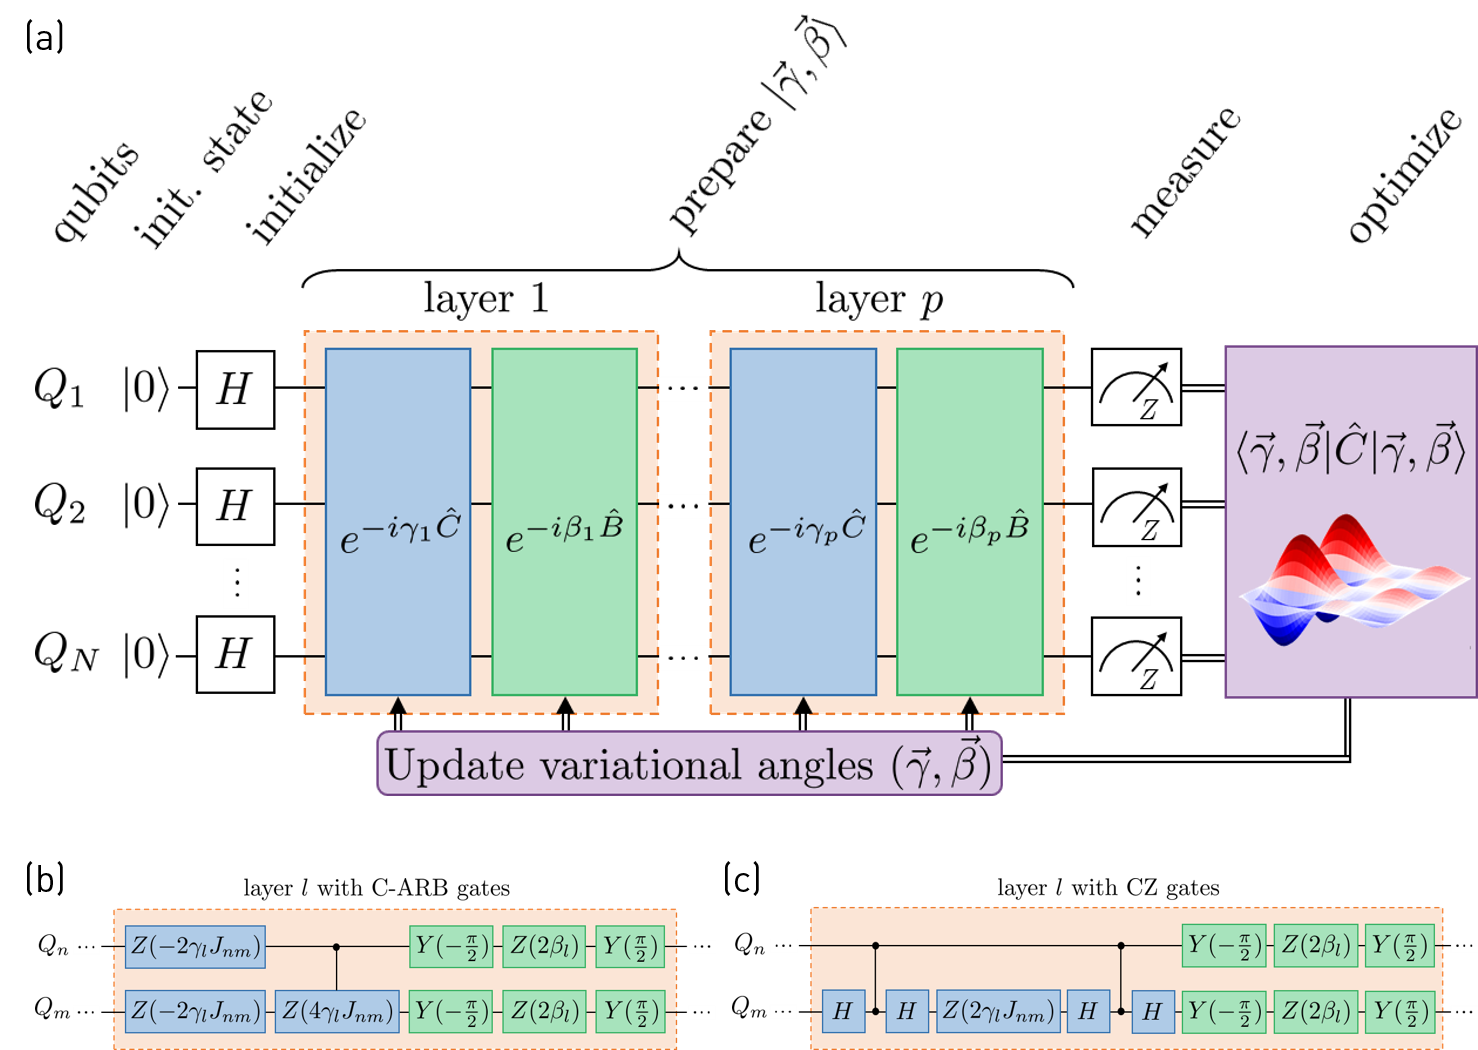
\includegraphics[width=\textwidth]{chapters/qaoa/figs/qaoa_scheme.png}
    \caption{The \gls{qaoa} scheme. (a) The scheme consists of two steps. First, the quantum computer applies $p$ alternating sequences -- called layers -- of two Hamiltonians ($\hat C$ and $\hat B$) scaled by layer-dependent variational parameters to an equal superposition state. The resulting state, $\ket{\vec\gamma,\vec\beta}$, is prepared and measured several time to obtain an estimate for the expectation value of a cost function \cost, based on the expectation values of single and two qubit terms. Based on this estimate, a classical optimizer alters the variational parameters to minimize \cost. The output of the algorithm is the projection of state \optimalstate yielding an bit-string which cost is small. }
    \label{fig:qaoa_scheme}
\end{figure}
\subsection{The importance of depth}
The depth of a \gls{qaoa} implementation is defined as the number of layers, $p$, used for the state preparatation.

For $p \rightarrow \infty$, the \gls{qaoa} finds the global optimium of $C$ \cite{Farhi2014AAlgorithm}. Intuitively, this is because the \gls{qaoa} can be seen as a Trotterized approximation \cite{TrotterMathematics} of the quantum adiabatic algorithm \cite{Farhi2000QuantumEvolution}. Similarly to the \gls{qaoa}, the quantum adiabatic algorithm starts in the highest energy state of the mixing Hamiltonian $\hat B$, i.e. equal superposition over all qubits in the $Z$ basis, and then evolves adiabatically to the cost Hamiltonian $\hat C$,
\begin{equation} \label{eq:qaoa_adiabatic_evolution}
\sexp{-\i \hat H(t)\,t}= \sexp{-\i \left(\hat H_1(t) +\, \hat H_2(t)\right) \, t} = \sexp{-\i \left((1-t / T) \hat B+ \, (t / T) \hat C\right)\, t}
\end{equation}
where $T$ is a real and positive parameter called run time. As long as the evolution is sufficiently slow i.e. $T$ is sufficiently large, this process forces the state of the system to remain in the ground state of the slowly varying Hamiltonian $\hat H(t)$, ultimately resulting to the ground state of $\hat C$ \cite{Farhi2000QuantumEvolution, Farhi2014AAlgorithm}. \gls{qaoa} is a trotterized approximation of this evolution, where the Trotter product formula stipulates that for two \textit{time independent} Hamiltonians $\hat H_1$ and $\hat H_2$ \cite{TrotterMathematics}:
\begin{equation} \label{eq:qaoa_product_formula}
    \sexp{-\i\left(\hat H_{1} + \hat H_{2}\right) t}=\lim _{K \rightarrow \infty}\left(\sexp{-\i \hat H_{1} t / K} \sexp{-\i \hat H_{2} t / K}\right)^{K}
\end{equation}
Truncating this equation to a finite value for  $K$ yields an error $\epsilon$ with lowest order term in $\mathcal{O}\left(\frac{t^2}{2K} [\hat H_1, \hat H_2]\right)$ \cite{Heyl2018QuantumSimulation, Lloyd1996UniversalSimulators}.

To relate this forumla to the time evolution of Eq. \eqref{eq:qaoa_adiabatic_evolution}, we approximate $\hat H_1(t)$ and $\hat H_2(t)$ by piecewise constant Hamiltionians that take the value $\hat H_i(l\Delta \tau)$ for $i = 1,2$ over intervals of length $\Delta \tau$ such that
\begin{equation} \label{eq:qaoa_discretization}
    \sexp{-\i\left(\hat H_{1}(t) + \hat H_{2}(t)\right) t} \approx \prod_{l = 1}^L \sexp{-\i\left(\hat H_{1}(l\,\Delta \tau) + \hat H_{2}(l\,\Delta \tau)\right) t}
\end{equation}
This approximation is valid as long as $\Delta \tau \ll\|\partial \hat H(t) / \partial t\|^{-1}$ \cite{Poulin2011QuantumSpace}, namely as long as time fluctuations in $H$ are small on the interval $\Delta \tau$.

Then, we use Eq. \eqref{eq:qaoa_product_formula} with $K = 1$ to decompose each matrix exponential,
\begin{equation}
    \sexp{-\i\left(\hat H_{1}(l\,\Delta \tau) + \hat H_{2}(l\,\Delta \tau)\right) t} = \sexp{-\i\hat H_{1}(l\,\Delta \tau)t}\cdot \sexp{\hat H_{2}(l\,\Delta \tau) t} + \epsilon 
\end{equation}
Combinating this first order trotter approximation with  Eq. \eqref{eq:qaoa_discretization} and Eq. \eqref{eq:qaoa_adiabatic_evolution} yields for the full time evolution:
\begin{equation}
    \prod_{l=1}^L\sexp{-\i\overbrace{(1-l\Delta\tau/T)\Delta\tau}^{\gamma_l}\hat C} \cdot \sexp{-\i\overbrace{(l\Delta\tau/T)\Delta\tau}^{\beta_l}\hat B} 
\end{equation}

PROBLEM: C and B are in reversed order. so last equation does not work, also should define $U(t1, t2) $ to indicate evolution from t1 to t2. 

have more layers = longer run time T for fixed delta t (or shorter delta t for same run time?)


\subsection{Speedup}
At the time of its publication, the \gls{qaoa} achieved a higher approximation ratio on MAX-3-LIN-2 -- a specific instance of the NP-complete MaxCut problem \cite{GareyM1990} -- than any other classical algorithm. This is no longer the case \cite{Barak2015BeatingDegree, Hastings2019CLASSICALALGORITHMS}. In fact, several work have shown that classical algorithms could outperform the \gls{qaoa} on a variety of problem instances \cite{Barak2015BeatingDegree, Hastings2019CLASSICALALGORITHMS, Bravyi2019ObstaclesProtection}. On the other hand, several work claim to achieve Grover speedup for unstructured search \cite{Jiang2017Near-optimalField} and state transfer \cite{Niu2019OptimizingDepth}. Whether or not the \gls{qaoa} will provide a provable or practical speedup compared to classical algorithms remains an open research question.

Nevertheless, the \gls{qaoa} remains one of the most studied \gls{vqa} in literature -- both theoretically and experimentally. It is therefore a good candidate to illustrate the advantage of \glspl{carb} and compare their performance with other published experiments. 


- introduced by Farhi, extension to ansatz
- scaling, why we want it
- idea of two non commuting hamiltonians
- trotterization : https://vtomole.com/blog/2019/04/07/trotter 
- explain flow
- role of p
- work on influence of p for large problems
- christian scaling of p with number of qubits
\subsection{Success probability}
Measuring successive preparations of \optimalstate yields a distribution of projected states $\ket{\psi_i}$.
We define the success probability, $P_s$, as the probability of measuring a projected state that is a solution to the combinatorial problem. 

Note that the optimization is performed on the smooth landscape of \cost{} and not on $P_s$ directly. But for problems with discrete domain of real values, a low expectation value of the cost function generally guarantees a high concentration of probability on optimal solutions upon measurement \cite{Cook2019TheCover, Wang2019XY-mixers:QAOA}.

\subsection{Cost hamiltonian with CZ/CARB}



\section{Experiment}
In this section, we implement the \gls{qaoa} on a quantum processor to find an approximate solution to a combinatorial optimization problem with 3 qubits. We use qubits 1, 2 and 3 of the device presended in Appendix \ref{app:device}. Information relative to the single- and two-qubit gates are reported in Appendix \ref{app:gate_parameters}. All measurements are performed with 3-level single shot readout

After introducing the combinatorial problem, we assess how the direct and decomposed implementations of the arbitrary phase gate affect the performance of the algorithm for different depths. We show that the direct implementation allows to solve the problem more effectively than the decomposed implementation, because more layers can be implemented for a fixed length. 

\subsection{Exact cover: definition and example problem instance}
We use \gls{qaoa} to find an approximate solution to an instance of the exact cover problem. The exact cover \cite{Karp1972ReducibilityProblems} is an NP-complete \cite{GareyM1990} decision problem formulated as follow: \textit{given a set $\mathcal{N}$, and a collection $\mathcal{L}$ of subsets of $\mathcal{N}$, is there a subcollection $\mathcal{L}'$ of $\mathcal{L}$ for which each element in $\mathcal{N}$ is included exactly once?} In other words, elements of the subcollection $\mathcal{L}'$ must be disjoint and their union must be $\mathcal{N}$.

As mentioned in Section \ref{sec:qaoa}, any NP-complete can be mapped onto an Ising Hamiltonian in polynomial time. For the exact cover, it is most conviently done using an incidence matrix $M$ \cite{WeissteinIncidenceMatrix}, where each row corresponds to an element of $\mathcal{L}$ and each column to an element of $\mathcal{N}$. The matrix element $M_{ln}$ is equal to 1 if the $l$-th element of $\mathcal{L}$ contains the $n$-th element of $\mathcal{N}$ and 0 otherwise.
The Ising parameters $J_{nl}$ and $h_l$ are obtained from $M$ \cite{Lucas2014IsingProblems, Vikstal2019ApplyingProblem}:
\begin{subequations}
\begin{equation}
    J_{l n}=\frac{1}{2} \sum_{k=1}^{N} M_{l k} M_{n k}
\end{equation}
\begin{equation}
h_{l}=\frac{1}{2} \sum_{n=1}^{N} M_{l n}\left(\sum_{k=1}^{L} M_{k n}-2\right)
\end{equation}
\end{subequations}
This formulation results in $L = |\mathcal{L}|$ spins in the Ising Hamiltionian, and each spin is mapped to a qubit. 

In this work, we consider the 3-qubit problem instance depicted in Fig. \ref{fig:qaoa_exact_cover_matrix}.  $\mathcal{N} := \{1,2,3\}$ and the elements of $\mathcal{L}$ are $A := \{1,2\},\,\, B := \{1,2,3\}$ and $C := \{2,3\}$, encoded in qubit 1, 2 and 3 respectively. In this picture, the decision problem becomes: \textit{is there a subcollection $\mathcal{L}'$ of letters for which each number in $\mathcal{N}$ is included exactly once?} The answer is yes, and the corresponding subcollections are $\mathcal{L}_1' = \{B\}$ and $\mathcal{L}_2' = \{A,C\}$. These subcollections are encoded in the states $\ket{\psi}=\ket{010}$ and $\ket{101}$, where a 1 in position $l$ indicates that the $l$-th element of $\mathcal{L}$ is included in the subcollection $\mathcal{L'}$.

\begin{figure}[ht]
    \centering
    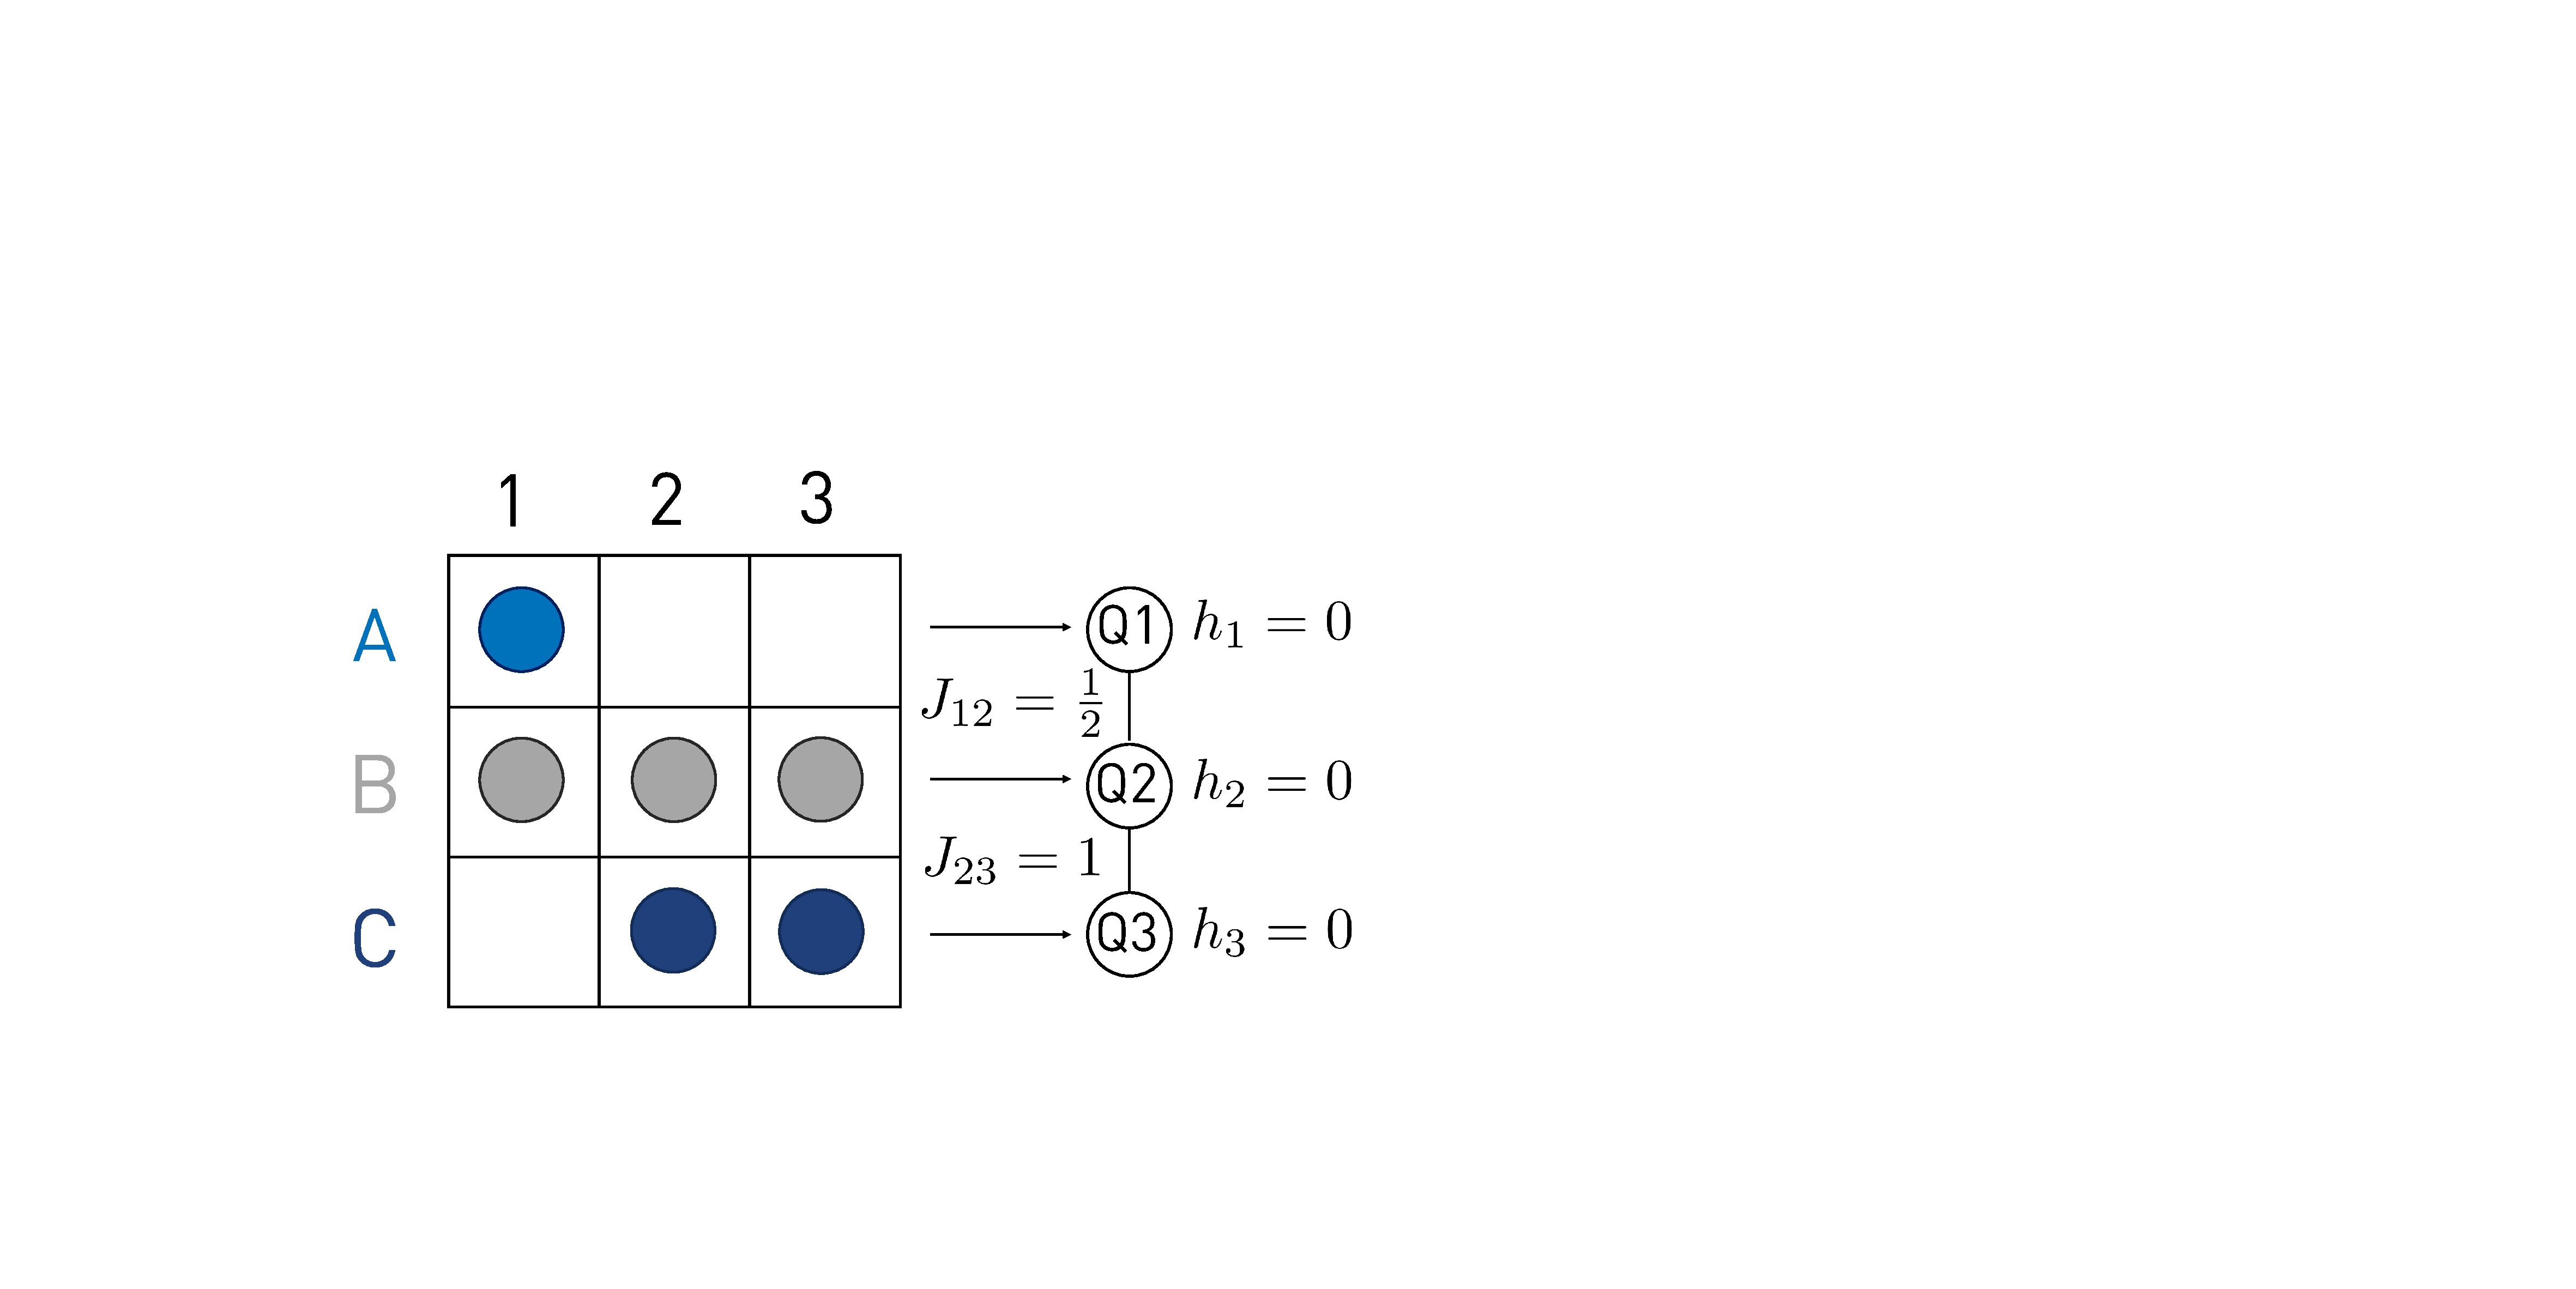
\includegraphics[width=\textwidth, trim={11cm 8cm 38cm 10cm},clip]{chapters/qaoa/figs/exact_cover_matrix.pdf}
    \caption{Incidence matrix representation of the exact cover problem instance implemented in this work. A dot in indicates a 1 and an empty square indicates a 0. The mapping to the 3 qubit chain and the corresponding Ising Hamiltonian parameters are indicated on the right handside.}
    \label{fig:qaoa_exact_cover_matrix}
\end{figure}

The resulting cost Hamiltonian is
\begin{equation}
    \hat C = \frac{1}{2}\hat\sigma_1^z\hat\sigma_2^z + \hat\sigma_2^z\hat\sigma_3^z
\end{equation}
and the corresponding cost function $\cost = \bra{\vec\gamma, \vec\beta} \hat C \qaoaMeasuredState{}$ reaches its minimum value of $-1.5$ when $\qaoaMeasuredState{} = \ket{101}$ or $\ket{010}$. 

From noise-free simulations of the unitary evolution combined with brute force optimization, we observe that the problem requires 3 layers to achieve a success probability larger than 99\%.

In the following sections, we present the results of the i
explain experiment and goal to compare both implementations
-refer to appendix for details about device and two qubit gates params
- describe that we remove leakage.

While 2\% is high for algorithms sensitive to leakage, it is not a major concern for QAOA, as long as the sequence

\section{Optimization landscapes ($p$ = 1)}
\begin{figure}[ht]
    \centering
    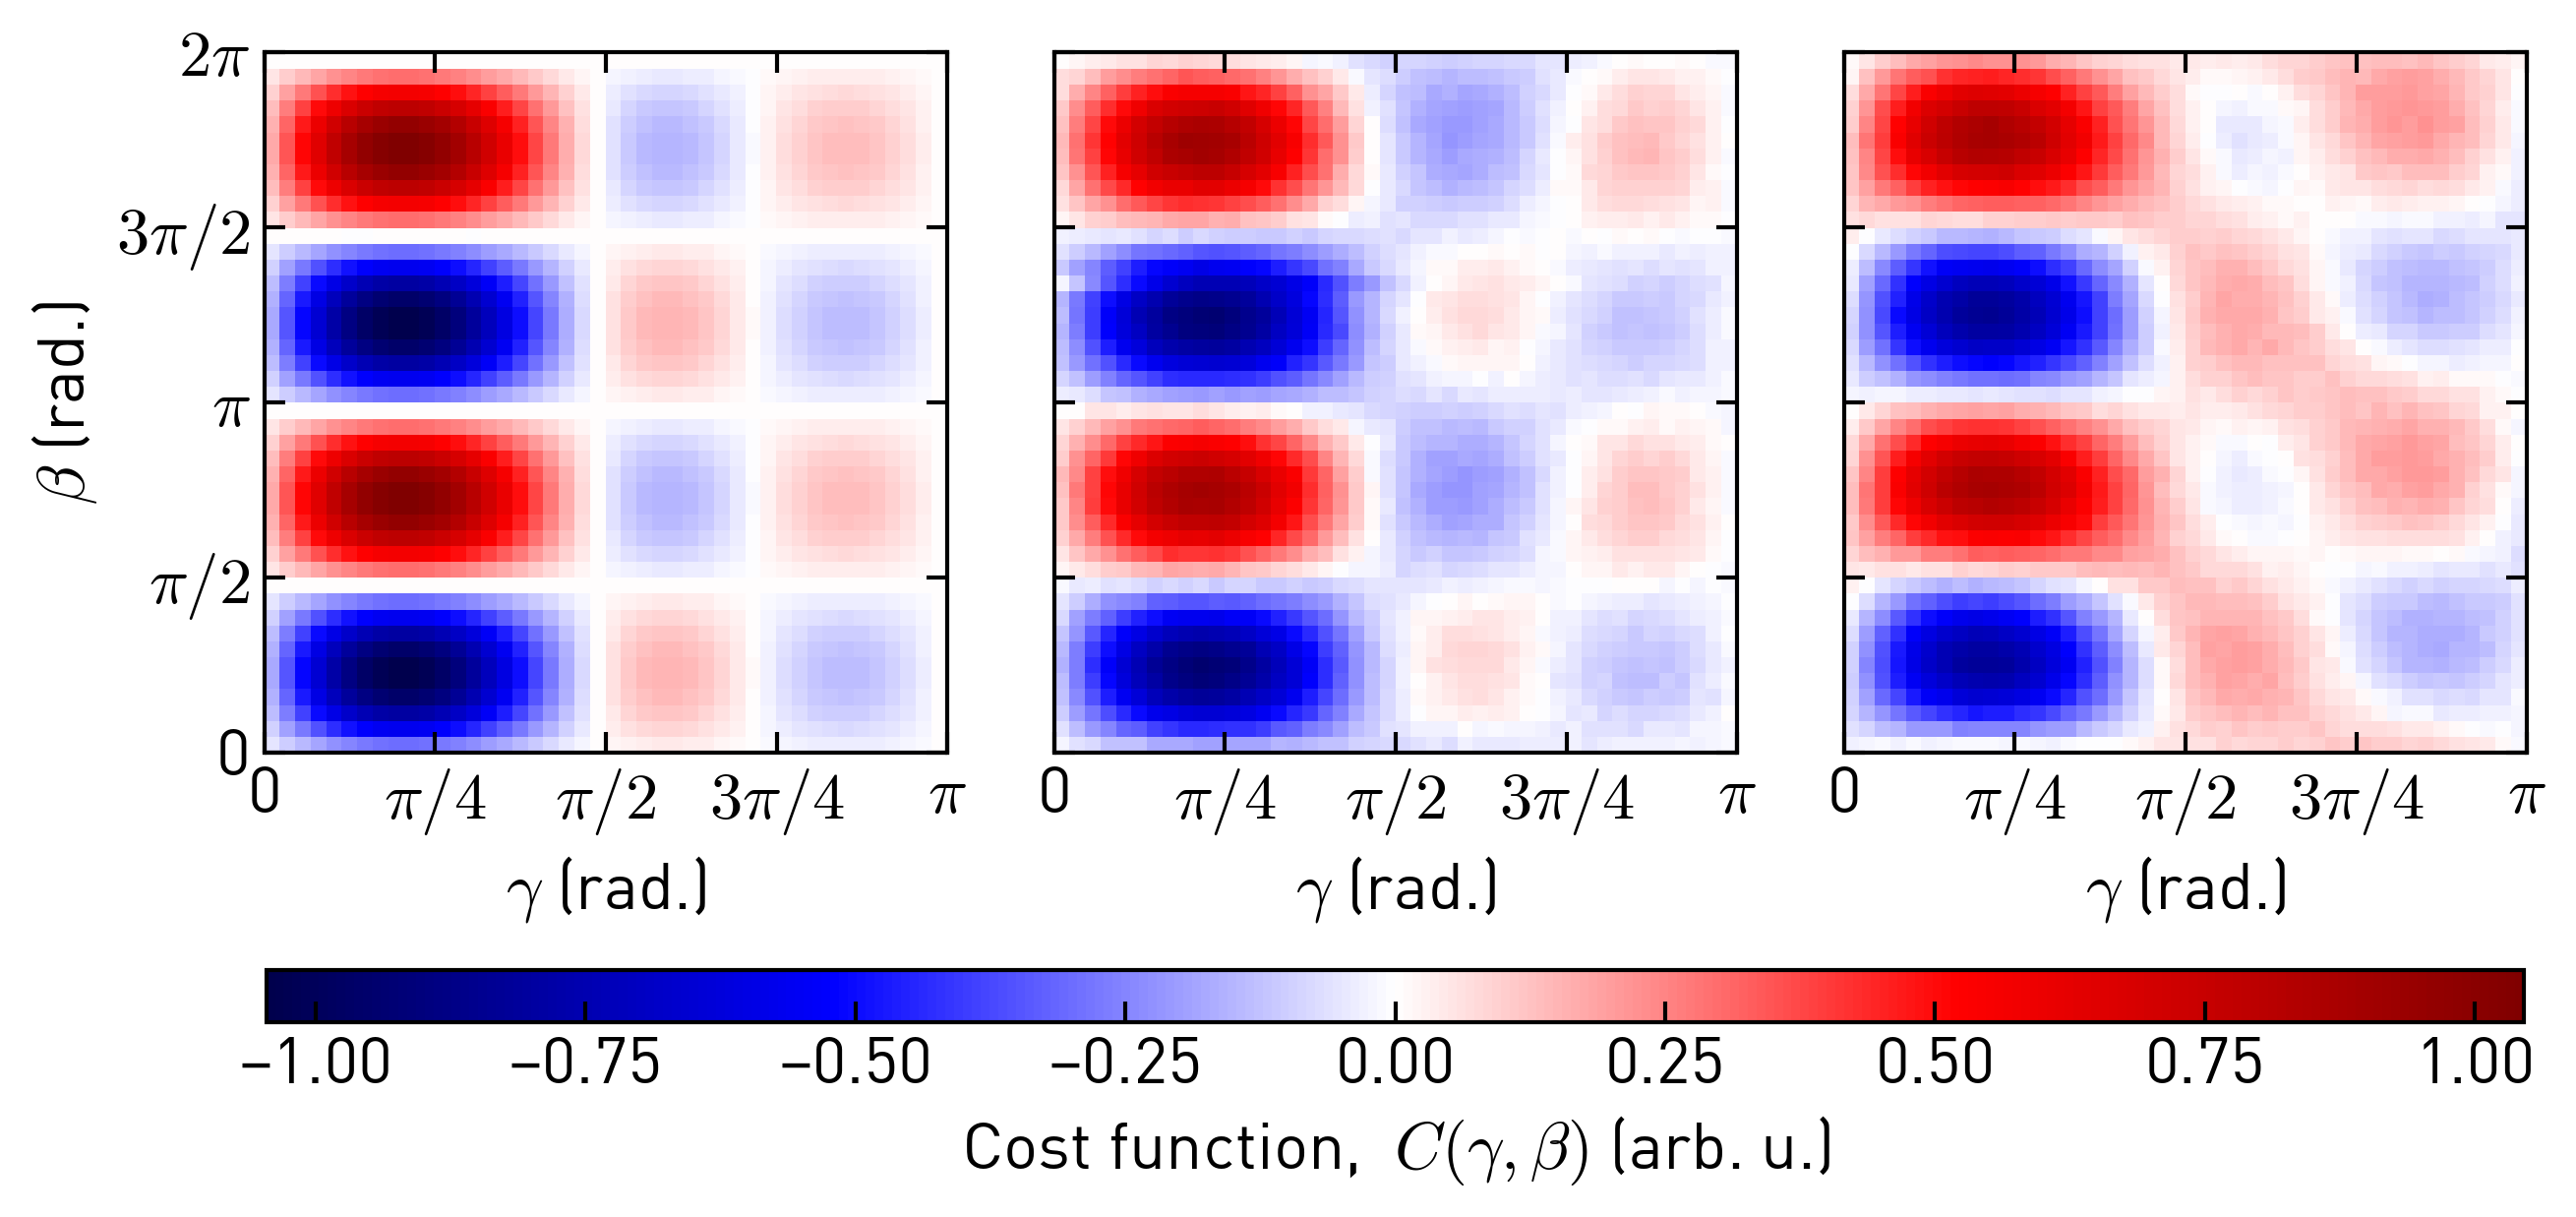
\includegraphics[width=\textwidth]{chapters/qaoa/figs/qaoa_landscapes_20200129_125251.png}
    \caption{Landscapes}
    \label{fig:qaoa_landscapes}
\end{figure}
- landscapes
- simulation
- local minimas
- intuition for parameters space shape

\section{Init from random}
\begin{figure}[ht]
    \centering
    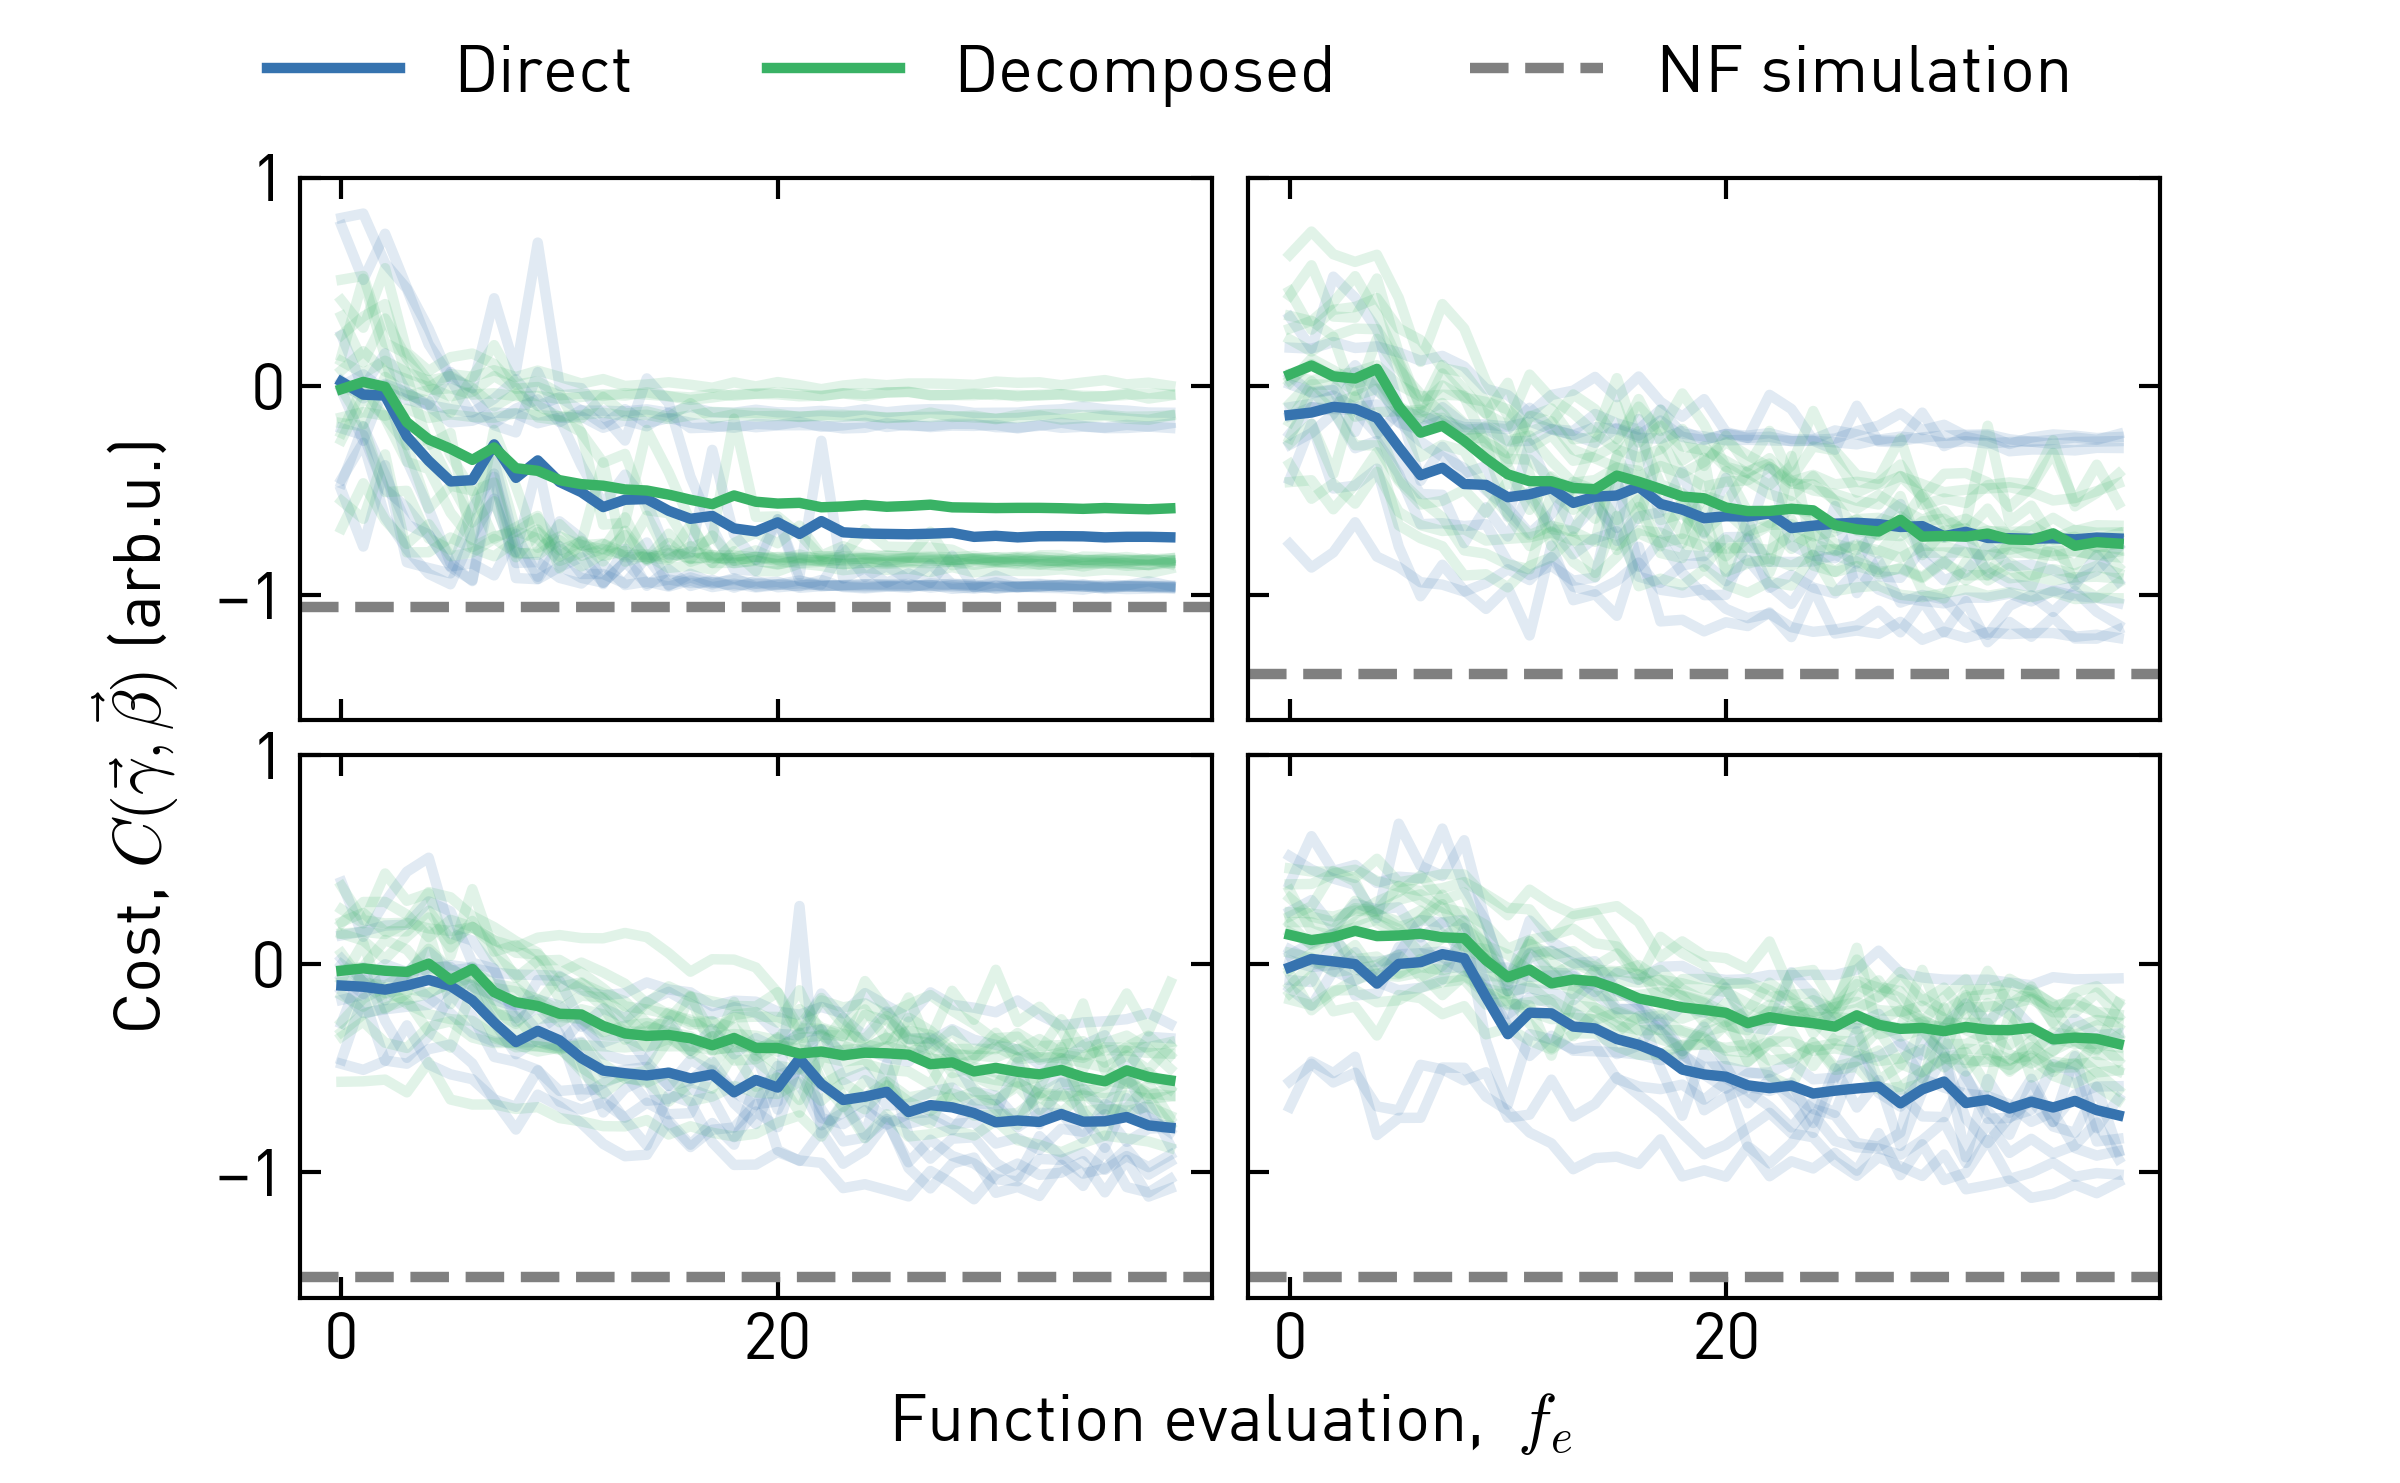
\includegraphics[width=\textwidth]{chapters/qaoa/figs/ch5_qaoa_optimization_traces_20200116_165916.png}
    \caption{Landscapes}
    \label{fig:qaoa_optimization_traces}
\end{figure}
- discuss optimizer, say what other used, what is important (low sampling, noise robust, avoid local minima)
- compare as function of p energy for both implementations

\section{Success prob as function of depth}


\begin{figure}[ht]
    \centering
    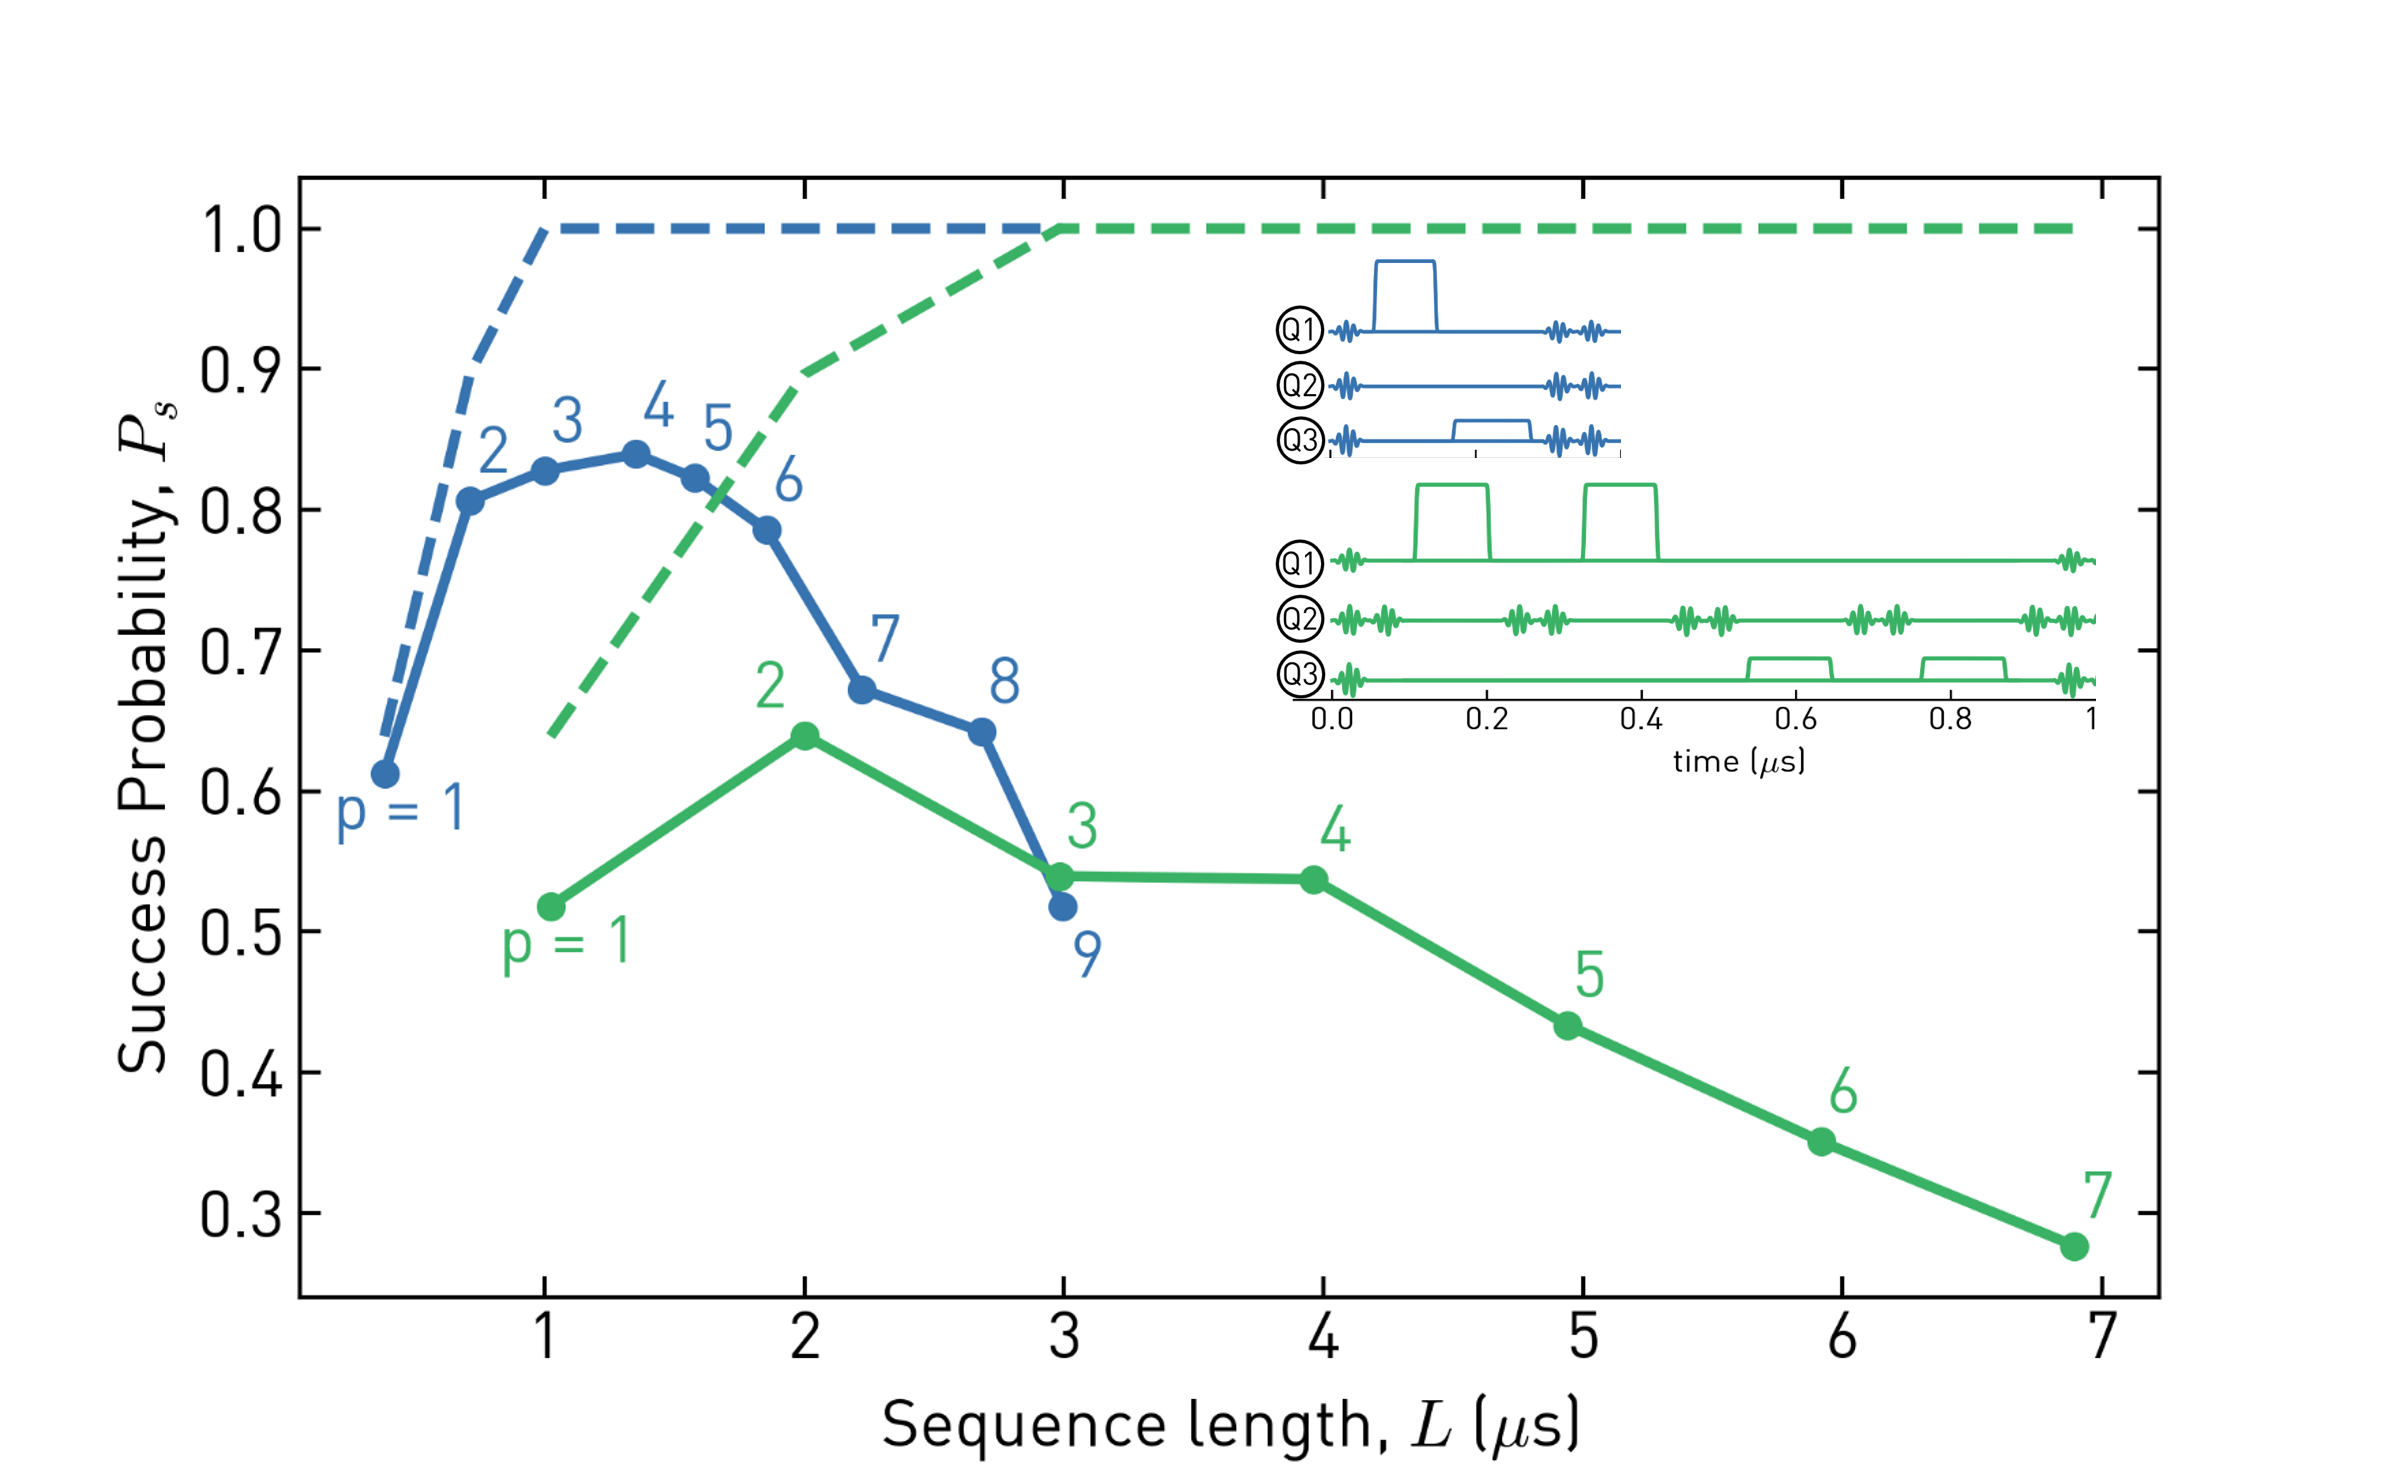
\includegraphics[width=\textwidth]{chapters/qaoa/figs/ch5_qaoa_sequence_lengths_v1_withinset_20200202_120000.png}
    \caption{Success probability as function of sequence length}
    \label{fig:qaoa_sequence_lengths}
\end{figure}

\begin{figure}[ht]
    \centering
    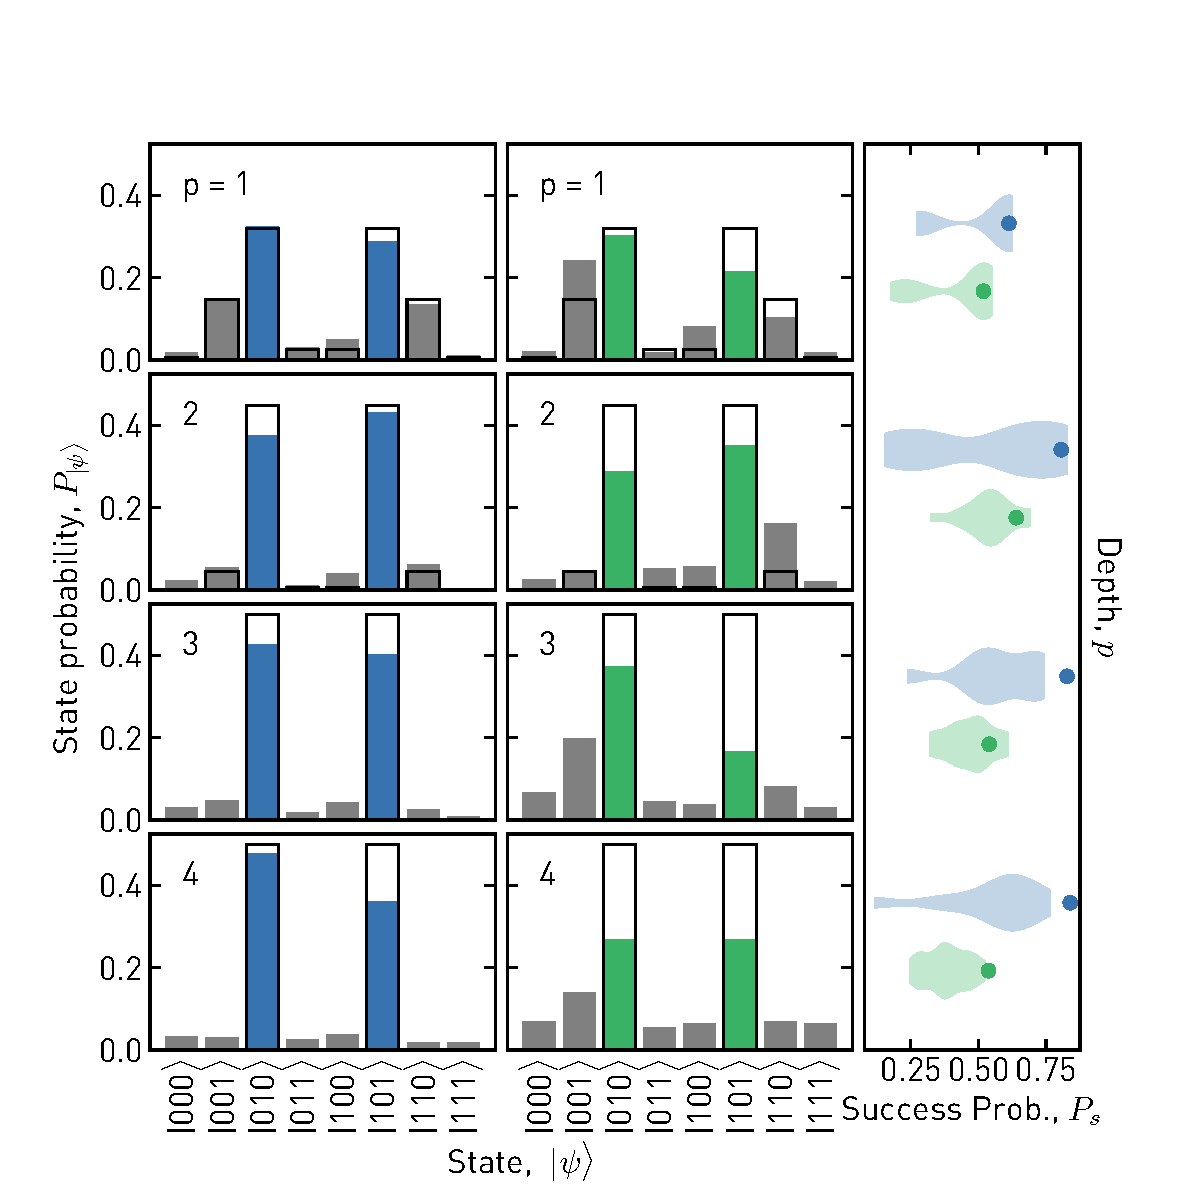
\includegraphics[width=\textwidth]{chapters/qaoa/figs/ch5_qaoa_state_histograms_20200202_134816.pdf}
    \caption{Landscapes}
    \label{fig:qaoa_state_histogram}
\end{figure}
\section{Conclusion}
